\documentclass[%handout,
	sans,
	12pt,
	%slidescentered,% center text on slide
	%draft,			% compile as draft version
	%notes,			% include nodes in slides
	%compress		% compress navigation bar
]{beamer}

\beamertemplatenavigationsymbolsempty

\setbeamertemplate{frametitle}
{
    \vspace*{1.5em}\insertframetitle\vspace*{-1.5em}
}

\usepackage[T1]{fontenc}
\usepackage[utf8x]{inputenc}

\usepackage{mathpazo}
\usepackage[british]{babel}
\usepackage{csquotes}

\usepackage{svg}

\newcommand{\high}[1]{{\usebeamercolor[fg]{structure} #1}}
\newcommand{\bad}[1]{\textcolor{red}{#1}}
\newcommand{\gray}[1]{\textcolor{darkgray}{#1}}
\newcommand{\black}[1]{\textcolor{black}{#1}}

\usepackage{amsmath,amssymb}
\usepackage{upgreek}
\usepackage{booktabs}
\usepackage{hyperref}
\usepackage{default}
\usepackage{graphicx}
\usepackage{colortbl}
\usepackage{url}
\usepackage{setspace}
\usepackage{wrapfig}
\usepackage{tabularx}
\usepackage{pgfplots}
\pgfplotsset{compat=1.9}
\usepackage{tikz}
\usepackage{pgfplotstable}

\setbeamertemplate{caption}[numbered]

\newcommand{\RR}{\mathbb{R}}
\newcommand{\NN}{\mathbb{N}}
\def\braces#1{[#1]}

%\definecolor{mybg}{rgb}{0.9,0.9,0.9}
\definecolor{mybg}{rgb}{1,1,1}
\setbeamercolor{background canvas}{bg=mybg}

\title{An executables specification of BDDs in Isabelle}
\author{\normalsize Max Haslbeck and Julius Michaelis}
\institute[]{\footnotesize Fakultät für Informatik\\TU München}
\date{\footnotesize 26 February 2016}

\begin{document}

\maketitle


\section{Introduction - BDDs}
\begin{frame}{Introduction - BDDs}
\begin{figure}[htbp]
  \centering
  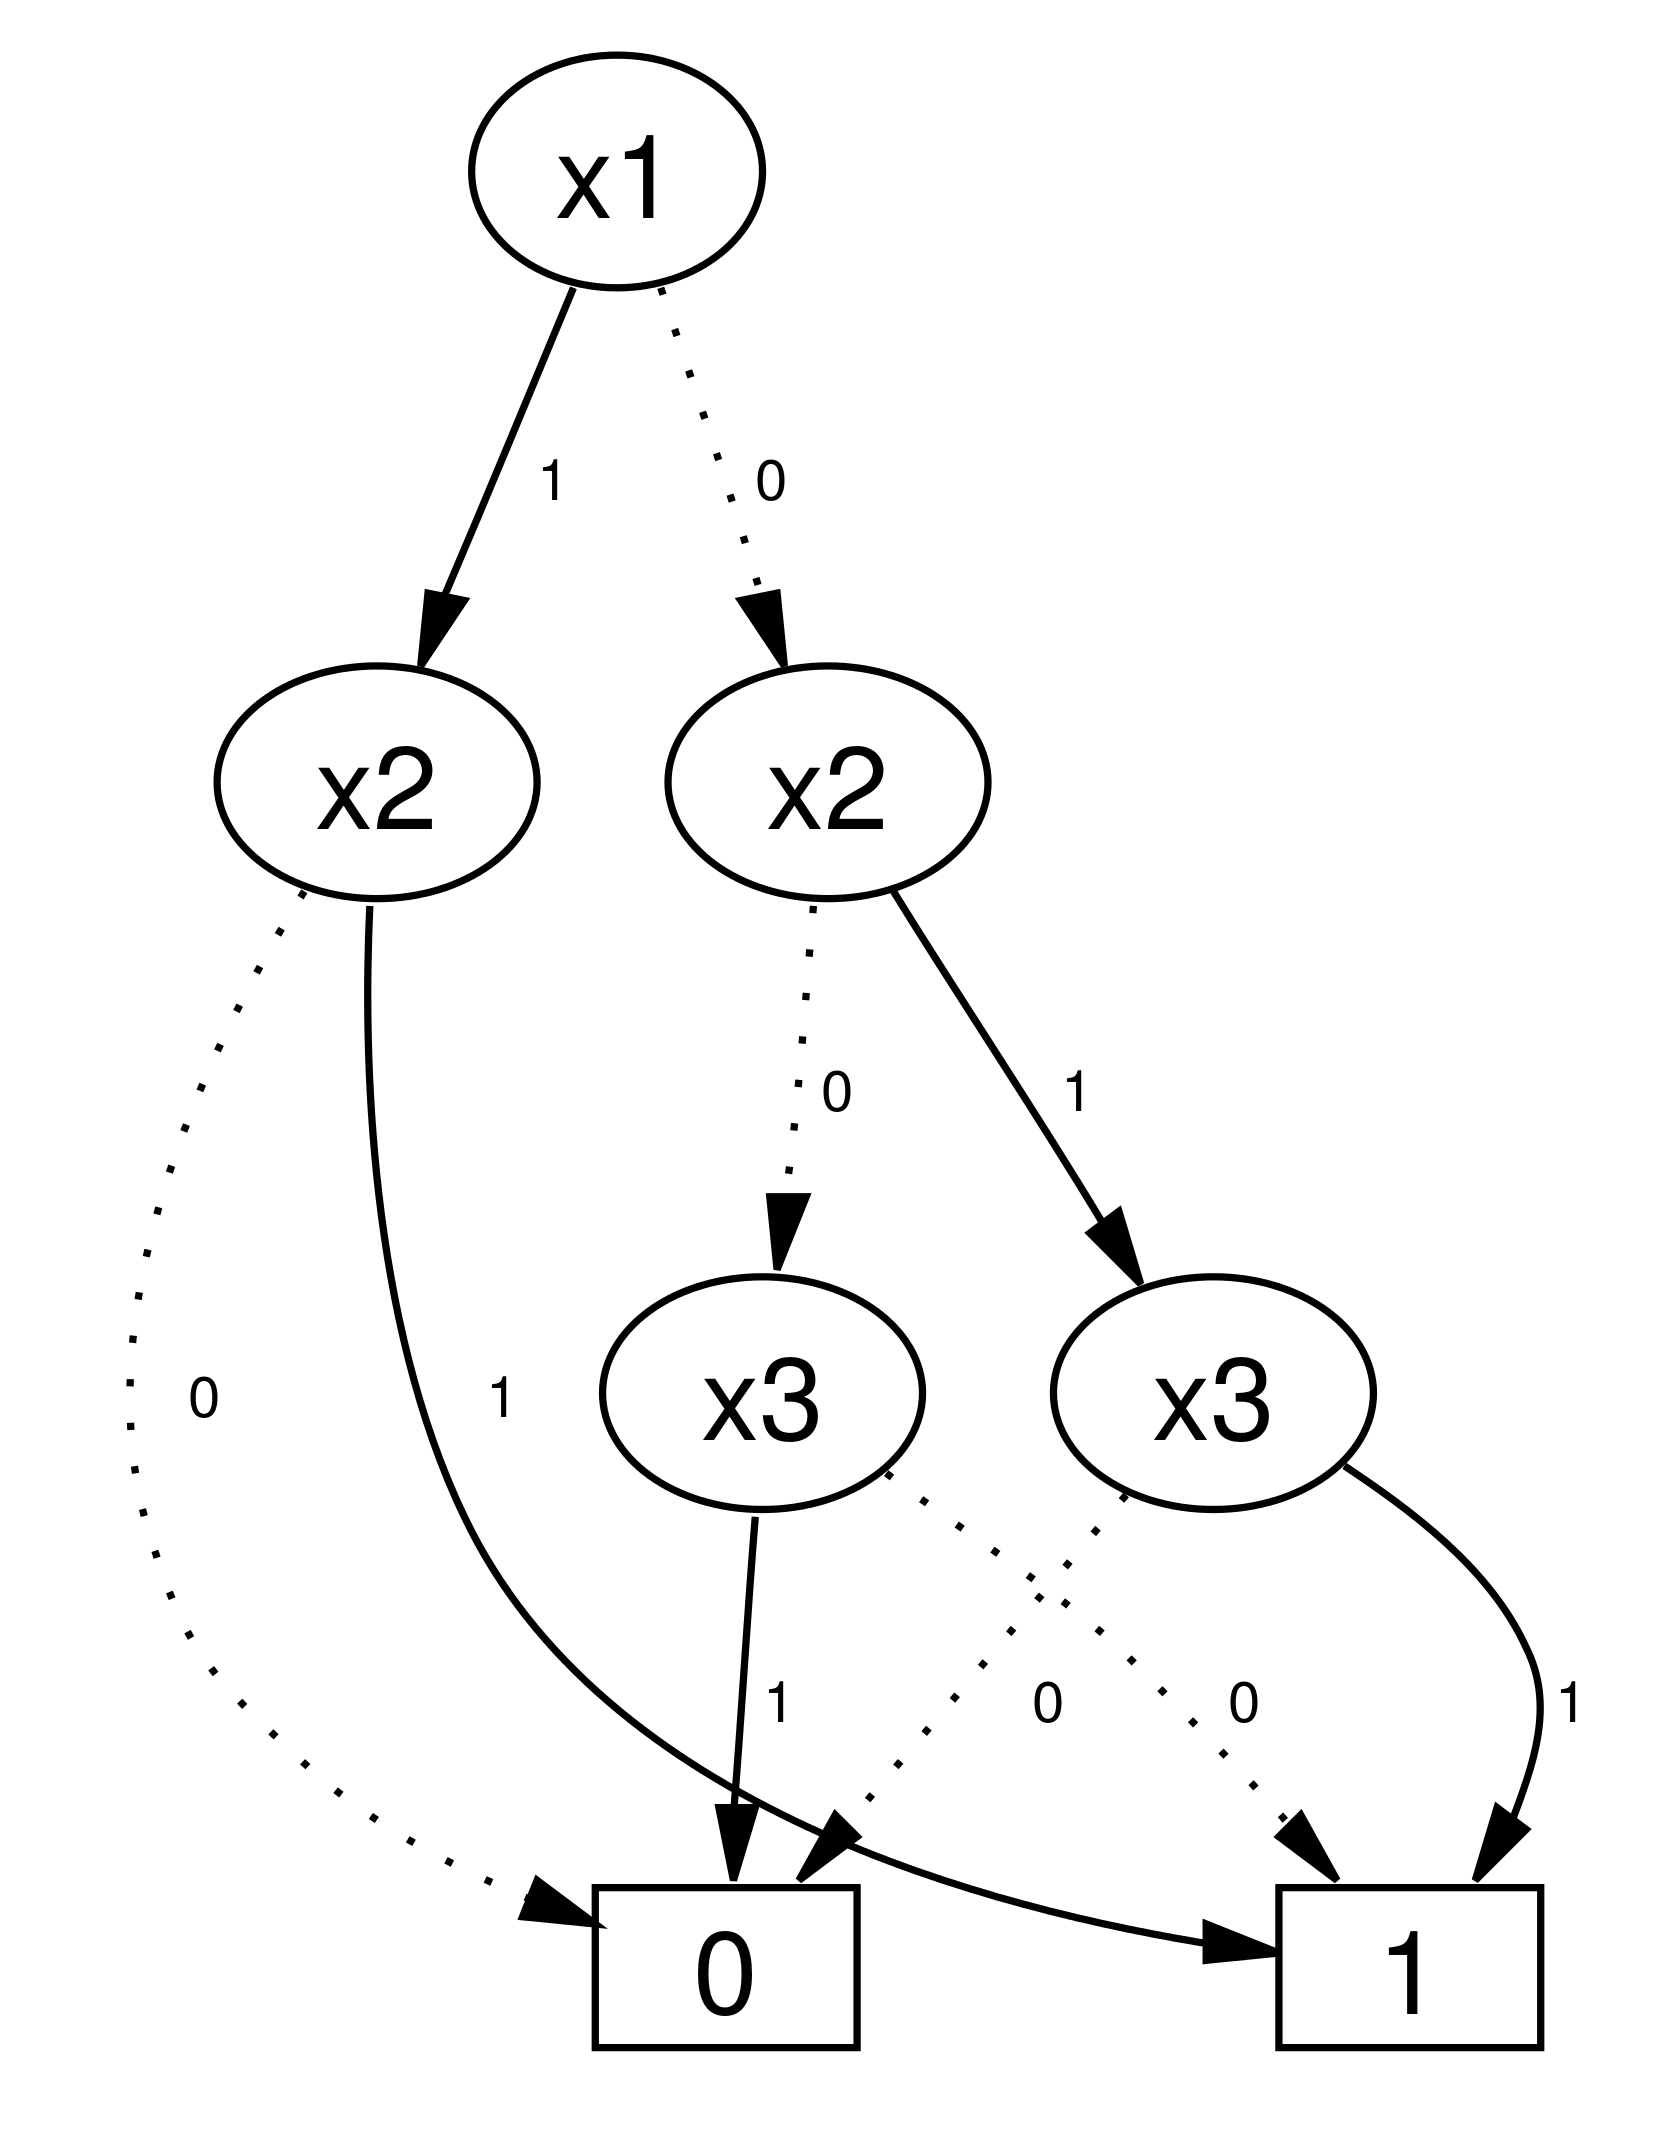
\includegraphics[height=5cm]{img/BDD_simple.png}
  \caption{BDD $(\overline{x_1} \land \overline{x_2} \land \overline{x_3}) \lor
           (x_1 \land x_2) \lor (x_2 \land x_3) $}
\end{figure}
  BDD = Binary Decision Diagram \\
  ROBDD = Reduced Ordered Binary Decision Diagram
\end{frame}


\begin{frame}{Boolean functions}
\begingroup
\addtolength{\jot}{-1mm}
{\footnotesize
\begin{flalign*}
    &\textbf{type\_synonym}\ \tau\ bf\ \textbf{=}\ (\tau \Rightarrow bool)
    \Rightarrow bool &
  \\[1\baselineskip]
    & \textbf{definition}\ \textit{bf-ite}\ ::\ \tau\ bf \Rightarrow
    \tau\ bf \Rightarrow \tau\ bf \Rightarrow \tau\ bf\ \textbf{where} &
  \\
    &\hskip4mm   \textit{bf-ite}\ i\ t\ e\ =\ (\lambda x.\ \text{if}\ i\ x\
    \text{then}\ t\ x\ \text{else}\ e\ x)&
  \\[1\baselineskip]
    &\textbf{definition}\ \textit{bf-restrict}\ ::\ \tau\ bf \Rightarrow \tau
    \Rightarrow bool \Rightarrow \tau\ bf\ \textbf{where}&
  \\
    &\hskip4mm \textit{bf-restrict}\ f\ v\ b\ =\ (\lambda a.\ f\ (a(v := b))&
  \\[1\baselineskip]
    & \textbf{lemma:}\ \textit{bf-ite}\ I\ T\ E\ =&
  \\
    &\phantom{\textbf{lemma:}}\ \textit{bf-ite}\ (\lambda l.\ l\ v)&
  \\
    &\phantom{\textbf{lemma:}\ \textit{bf-ite}}\
    (\textit{bf-ite}\ (\textit{bf-restrict}\ I\ v\ \textit{True})\
    (\textit{bf-restrict}\ T\ v\ \textit{True})&
  \\
    &\phantom{\textbf{lemma:}\ \textit{bf-ite}\ (\textit{bf-ite}}\
    (\textit{bf-restrict}\ E\ v\ \textit{True}))&
  \\
    &\phantom{\textbf{lemma:}\ \textit{bf-ite}}\
    (\textit{bf-ite}\ (\textit{bf-restrict}\ I\ v\ \textit{False})\
    (\textit{bf-restrict}\ T\ v\ \textit{False})&
  \\
    &\phantom{\textbf{lemma:}\ \textit{bf-ite}\ (\textit{bf-ite}}\
    (\textit{bf-restrict}\ E\ v\ \textit{False}))&
\end{flalign*}
}
\endgroup
\vspace*{-10mm}
\end{frame}


\begin{frame}{Binary Decision Trees}
\begingroup
\addtolength{\jot}{-1mm}
{\footnotesize
\begin{flalign*}
    &\textbf{datatype}\ (\tau :: \textit{linorder})\ \textit{bdt}\ \textbf{=}\
    \textit{Trueif}\ |\ \textit{Falseif}\ |\ IF\ \tau\ (\tau\ \textit{bdt})\
    (\tau\ \textit{bdt}) &
  \\[\baselineskip]
  &\textbf{definition}\
    \textit{bf-bdt-rel}\ = \{(bf, bd).\ \textit{ro-bdt}\ bd\ \land\ \forall a.\
    bf\ a = \textit{val-bdt}\ bd\ a\} &
  \\[\baselineskip]
    & \textbf{lemma:}\
    (bf,bd) \in \textit{bf-bdt-rel} \Longrightarrow (bf',bd') \in
    \textit{bf-bdt-rel}& \\ & \phantom{lemma:}\ \Longrightarrow  (bf = bf')
    \leftrightarrow (bd = bd') &
  \\[\baselineskip]
    &\textbf{lemma:}\ (i,ibd) \in
    \textit{bf-bdt-rel} \Longrightarrow (t,tbd) \in \textit{bf-bdt-rel}&
  \\
    &\phantom{lemma:}\Longrightarrow (e,ebd) \in \textit{bf-bdt-rel} & \\ &
    \phantom{lemma:}\Longrightarrow (\textit{bf-ite}\ i\ t\ e, \textit{bdt-ite}\
    ibd\ tbd\ ebd) \in \textit{bf-bdt-rel}&
\end{flalign*}
}
\endgroup
\vspace*{-10mm}
\end{frame}


\begin{frame}{Binary Decision Trees} % Maybe not necessary
\begin{figure}[htbp]
  TODO: Add image of our Binary decision tree
\end{figure}
\end{frame}


\begin{frame}{BDDs on abstract datatypes}
\begin{itemize}
  \item usage of Isabelle's locale feature
    \begin{itemize}
      \item define basic operations and respective assumptions
      \item Relation \textit{bdt-bdd-rel}
      \item $ (ib, ibd) \in \textit{bdt-bdd-rel}  \Longrightarrow $ \\
            $(tb, tbd) \in \textit{bdt-bdd-rel} \Longrightarrow $ \\
            $(eb, ebd) \in \textit{bdt-bdd-rel} \Longrightarrow $ \\
            $(\textit{bdt-ite}\ ib\ tb\ eb, \textit{bdd-ite}\ ibd\ tbd\ ebd)
             \in \textit{bdt-bdd-rel} $
    \end{itemize}
  \item instantiation of locale with abstract datatype \textit{pointermap}
\end{itemize}
\end{frame}


\begin{frame}{Implementation}
\begingroup
\addtolength{\jot}{-1mm}
{\footnotesize
\begin{flalign*}
  %TODO: Fugly hack to move to the right
  &\hskip1cm\textbf{record}\ \tau\ \textit{pointermap-impl} =&
  \\
  %TODO: Im to stupid for correct alignment, whitespace FTW
  &\hskip12mm \textit{entriesi}\ \ \ ::\ \tau\ \textit{array-list}&
  \\
  &\hskip12mm \textit{getentryi}\ ::\ (\tau, nat)\ \textit{hashtable}&
\end{flalign*}
}
\endgroup
\vspace*{-10mm}
Verification via separation logic
\end{frame}


\begin{frame}{Pointermap}
\begin{itemize}
  \item given an element, it constructs a pointer (or small representation) to 
        that element. For equal elements it supplies an equal pointer
        %TODO: better formulation
  \item given a pointer, we can retrieve an element
\end{itemize}
\begingroup
\addtolength{\jot}{-1mm}
{\footnotesize
\begin{flalign*}
  %TODO: Fugly hack to move to the right
  &\hskip1cm\textbf{record}\ \tau\ \textit{pointermap} =& \\
  %TODO: Im to stupid for correct alignment, whitespace FTW
  &\hskip12mm \textit{entries}\ \ \ ::\ \tau\ \textit{list}& \\
  &\hskip12mm \textit{getentry}\ ::\ \tau\ \Rightarrow \textit{nat}\
  \textit{option}&
\end{flalign*}
}
\endgroup
\vspace*{-10mm}
\end{frame}


\begin{frame}{Urquhart benchmark}
  \begin{center}
	\begin{align*}
	x_1 \longleftrightarrow (x_2 \longleftrightarrow (\dots \longleftrightarrow (x_n \longleftrightarrow \\
	(x_1 \longleftrightarrow (x_2 \longleftrightarrow (\dots \longleftrightarrow x_n))))))
	\end{align*}

	\begin{tikzpicture}[scale=.9]
		\begin{axis}[ylabel=time in s, xlabel=n]
      %TODO: fix labels
			\addplot table [col sep=comma] {urquhart1500.csv};
			\addplot table [col sep=comma] {buddy_urquhart1500.csv};
		\end{axis}
	\end{tikzpicture}
  \end{center}
\end{frame}


\begin{frame}{Conclusion}
	\begin{block}{Limitations}
		\begin{itemize}
			\item No garbage collection
			\item No variable reordering
		\end{itemize}
	\end{block}
	\begin{block}{Achievements}
		\begin{itemize}
			\item About a factor of 10 faster than previous work on BDDs in Isabelle
			\item Haskell tool for tautology checking available
		\end{itemize}
	\end{block}
\end{frame}

\end{document}
